\documentclass[12pt]{article}
\usepackage[utf8]{inputenc}
\usepackage[backend=biber]{biblatex}
\usepackage[a4paper]{geometry}
\usepackage{amsmath}
\usepackage{amssymb}
\usepackage{array}
\usepackage{bm}
\usepackage{graphicx}
\usepackage[hidelinks]{hyperref}
\usepackage{paracol}
\usepackage{wrapfig}
\usepackage{xcolor}

\addbibresource{references.bib}
\geometry{a4paper, margin=1in}

\title{Reinforcement Learning: Report}
\author{}
\date{\today}
% \newcommand{\wordcount}{\begin{center}Word count (excl. footnotes, references, etc.): 2,123\end{center}}


\begin{document}
\maketitle
% \wordcount

\setcounter{tocdepth}{2}
\tableofcontents
\listoffigures
\thispagestyle{empty}
\setcounter{page}{0}
\newpage

\section{Environments}

\subsection{Gymnasium}

The \texttt{gym.Env} class can be subclassed to create new custom environments by
implementing the \texttt{step()}, \texttt{render()} and \texttt{reset()} methods.

A variable-size $n \times m$ grid world goal finding environment can thus be set up
with the starting position $(0, 0)$ encoded as \texttt{<},
the agent position encoded as \texttt{@},
free positions encoded as \texttt{.},
and the goal position $(n - 1, m - 1)$ encoded as \texttt{>}.
\autoref{fig:grid-world-goal-finding-env-visualize_episode} shows such a $5 \times 5$ environment rendered
in a human readable format.

\begin{wrapfigure}{r}{0.59\textwidth}
	\centering
	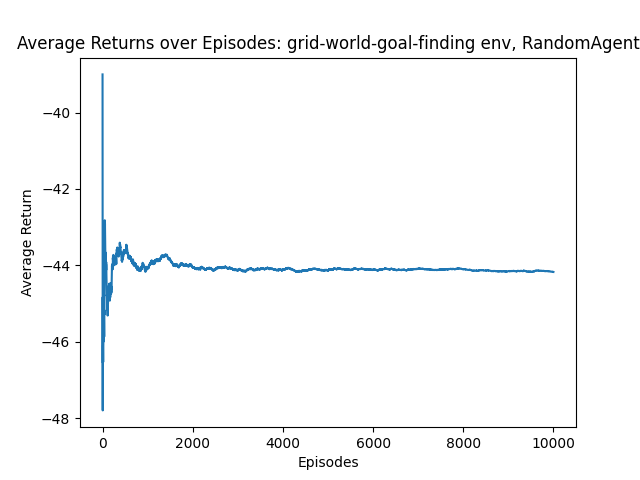
\includegraphics[width=0.57\textwidth]{figures/grid-world-goal-finding_average-returns.png}
	\caption{A random agent's average returns over 10,000 episodes in the $5 \times 5$ grid}
	\label{fig:grid-world-goal-finding_average-returns}
\end{wrapfigure}

The environment's action space consists of four actions: up, down, right, left.
For every action there is a negative reward of $-1$.
The agent will not move if it performs an action that would bring it off the grid,
but it still receives the negative reward of $-1$.

\autoref{fig:grid-world-goal-finding_average-returns} shows the average returns a random agent
accumulated in the grid world goal finding environment over 10,000 episodes, a \textit{quantitative}
way of evaluating the agent that smoothes out the spikes from the stochasticity of exploration:
the average returns are calculated as $\hat{G}_k = \frac{1}{k + 1} \sum_{i=0}^k{G_i}$,
where $G_k$ is the return at (zero-indexed) episode $k$.

\autoref{fig:grid-world-goal-finding-env-visualize_episode} shows the human readable rendering
of a 10-timestep episode with a random agent, a \textit{qualitative} way of evaluating an agent.

\begin{figure}[!h]
	\begin{verbatim}
Step 0:      Step 1:      Step 2:      Step 3:      Step 4:      Step 5:
@....        <....        <....        <....        <.@..        <@...
.....        @....        .@...        ..@..        .....        .....
.....        .....        .....        .....        .....        .....
.....        .....        .....        .....        .....        .....
....>        ....>        ....>        ....>        ....>        ....>

             Step 6:      Step 7:      Step 8:      Step 9:      Step 10:
             @....        <@...        <.@..        <.@..        <@...
             .....        .....        .....        .....        .....
             .....        .....        .....        .....        .....
             .....        .....        .....        .....        .....
             ....>        ....>        ....>        ....>        ....>
\end{verbatim}
	\caption{A random agent's trajectory in a $5 \times 5$ grid world 10-timestep episode}
	\label{fig:grid-world-goal-finding-env-visualize_episode}
\end{figure}

\subsection{Minihack}

Minihack provides more complex environments for an agent to interact with.
\autoref{fig:room-with-lava_FixedAgent} visualises 10 timesteps
of a fixed agent hard-coded to always move down and then right.

\begin{figure}[!h]
	\centering
	\begin{tabular}{ccccc}
		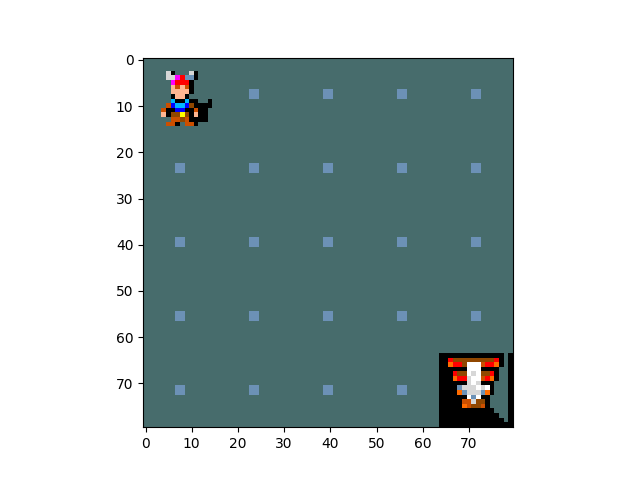
\includegraphics[width=0.18\textwidth]{figures/empty-room_FixedAgent/0.png} &
		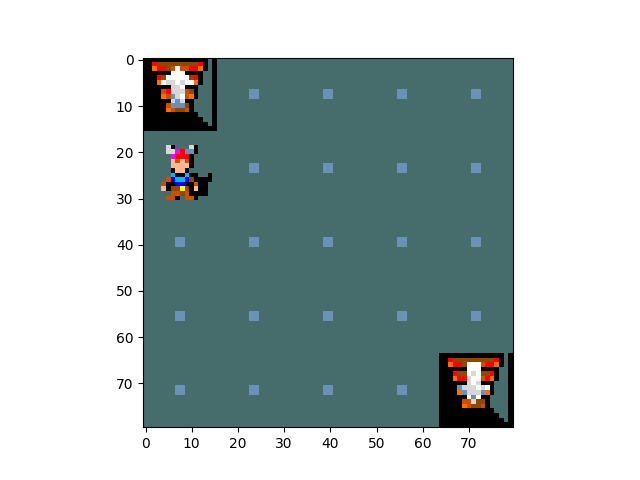
\includegraphics[width=0.18\textwidth]{figures/empty-room_FixedAgent/1.png} &
		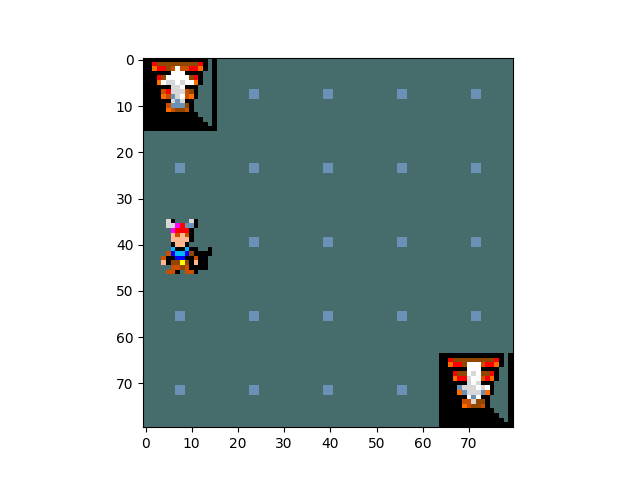
\includegraphics[width=0.18\textwidth]{figures/empty-room_FixedAgent/2.png} &
		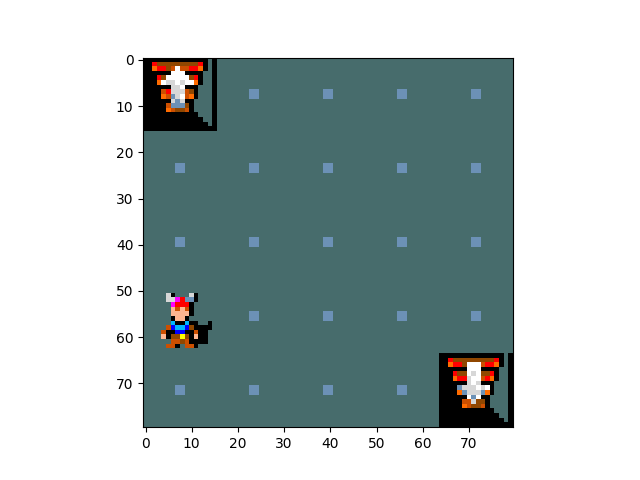
\includegraphics[width=0.18\textwidth]{figures/empty-room_FixedAgent/3.png} &
		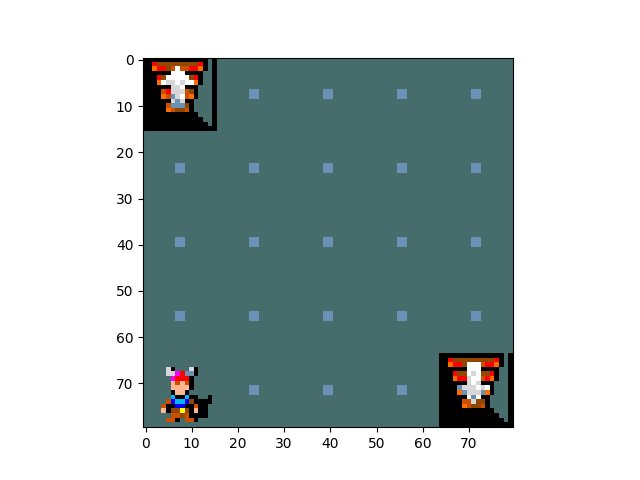
\includegraphics[width=0.18\textwidth]{figures/empty-room_FixedAgent/4.png}   \\
		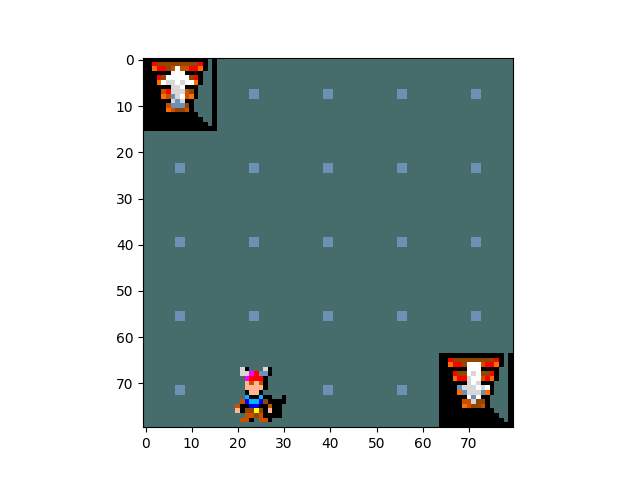
\includegraphics[width=0.18\textwidth]{figures/empty-room_FixedAgent/5.png} &
		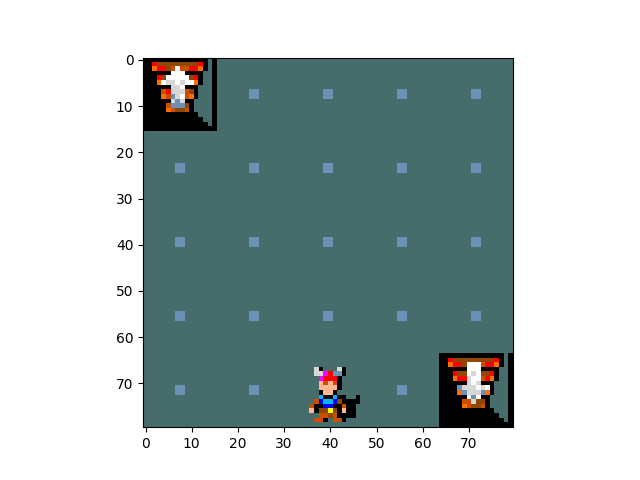
\includegraphics[width=0.18\textwidth]{figures/empty-room_FixedAgent/6.png} &
		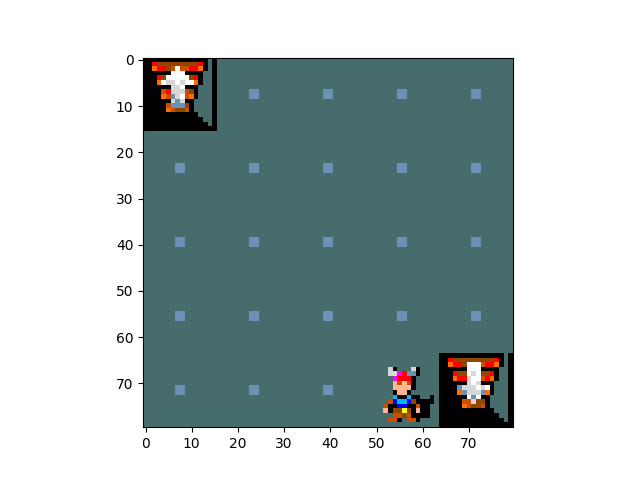
\includegraphics[width=0.18\textwidth]{figures/empty-room_FixedAgent/7.png} &
		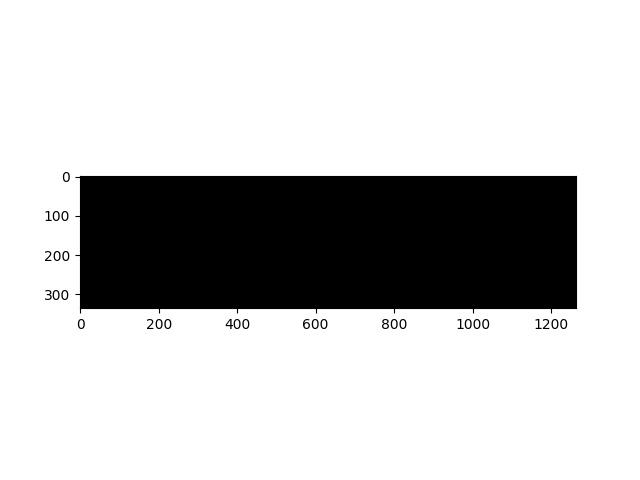
\includegraphics[width=0.18\textwidth]{figures/empty-room_FixedAgent/8.png}
	\end{tabular}
	\vspace{-20pt}
	\begin{tabular}{ccccc}
		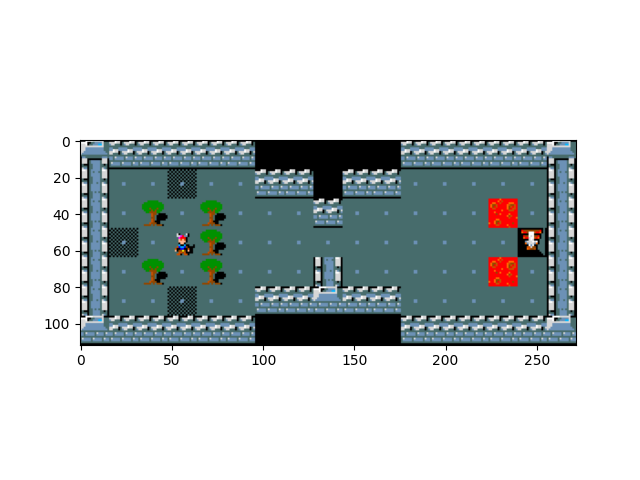
\includegraphics[width=0.18\textwidth]{figures/room-with-lava_FixedAgent/0.png} &
		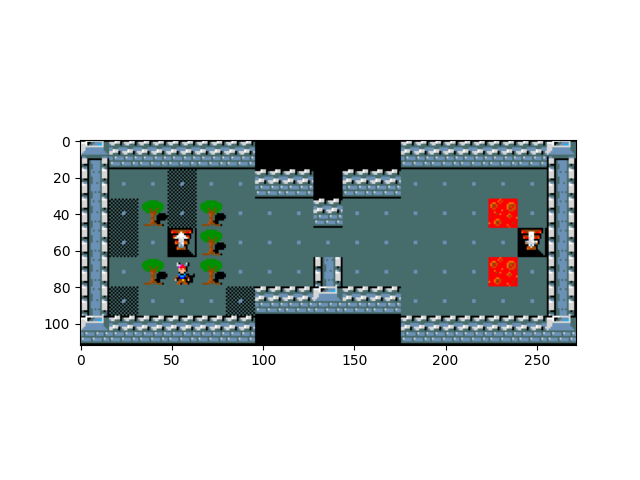
\includegraphics[width=0.18\textwidth]{figures/room-with-lava_FixedAgent/1.png} &
		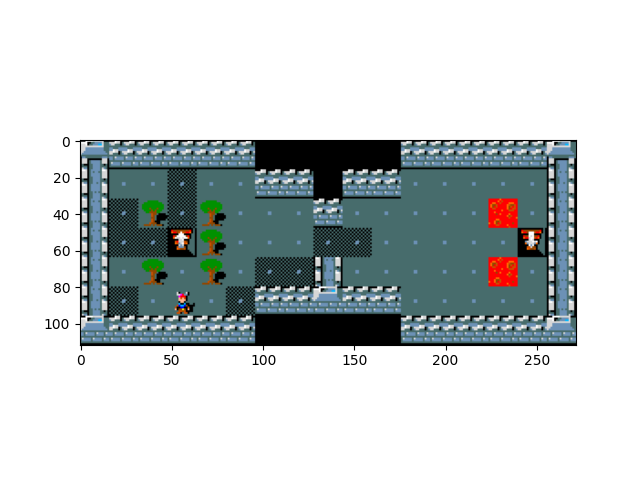
\includegraphics[width=0.18\textwidth]{figures/room-with-lava_FixedAgent/2.png} &
		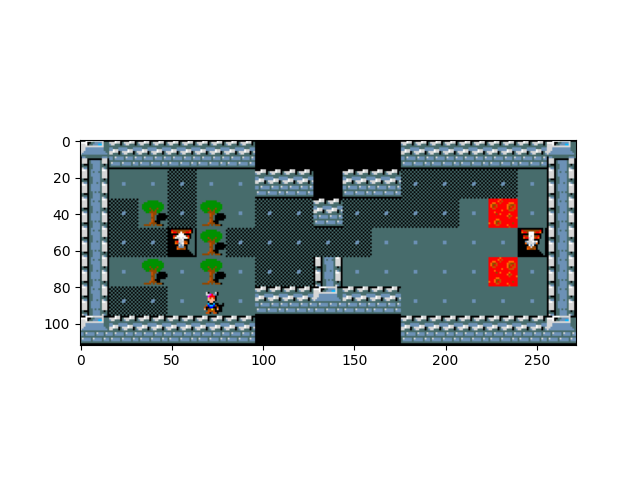
\includegraphics[width=0.18\textwidth]{figures/room-with-lava_FixedAgent/3.png} &
		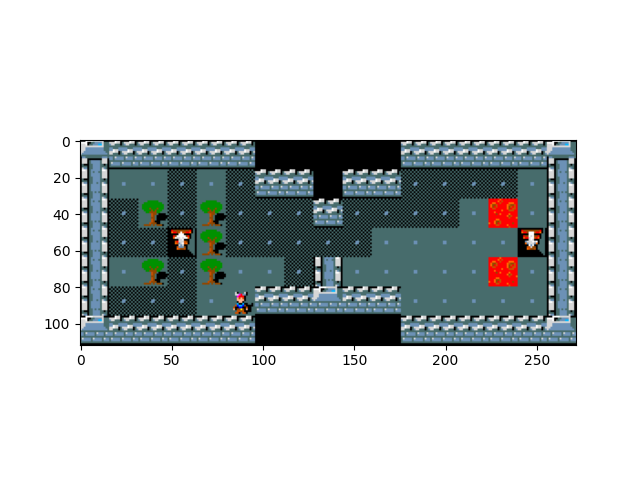
\includegraphics[width=0.18\textwidth]{figures/room-with-lava_FixedAgent/4.png}   \\
		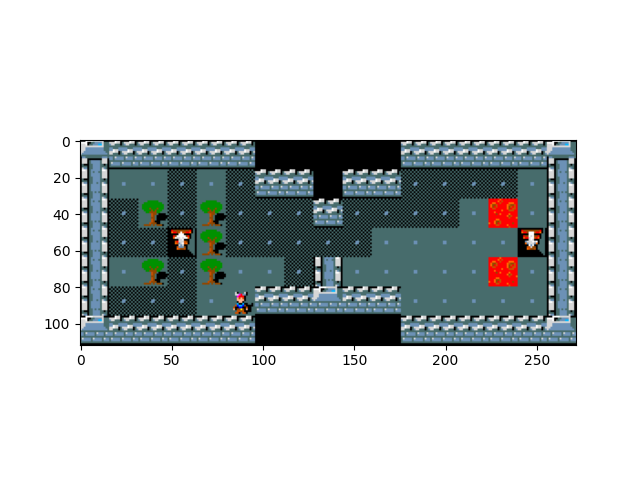
\includegraphics[width=0.18\textwidth]{figures/room-with-lava_FixedAgent/5.png} &
		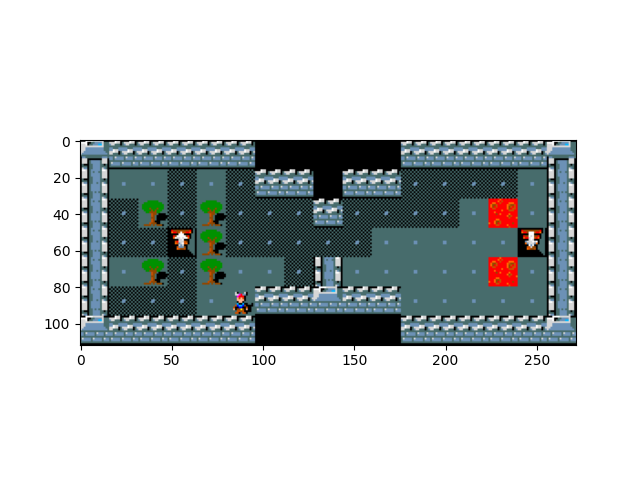
\includegraphics[width=0.18\textwidth]{figures/room-with-lava_FixedAgent/6.png} &
		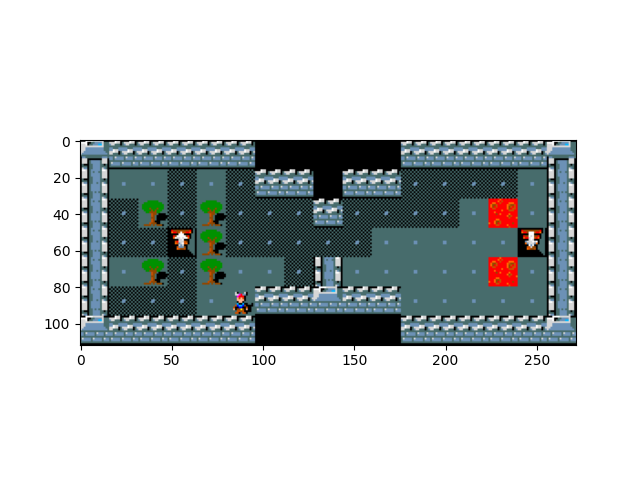
\includegraphics[width=0.18\textwidth]{figures/room-with-lava_FixedAgent/7.png} &
		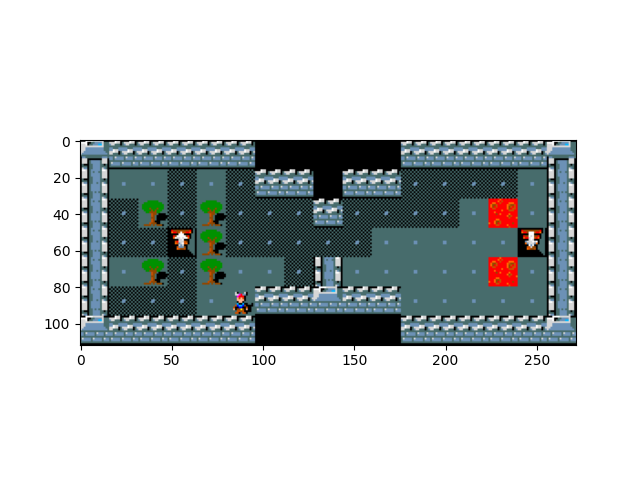
\includegraphics[width=0.18\textwidth]{figures/room-with-lava_FixedAgent/8.png} &
		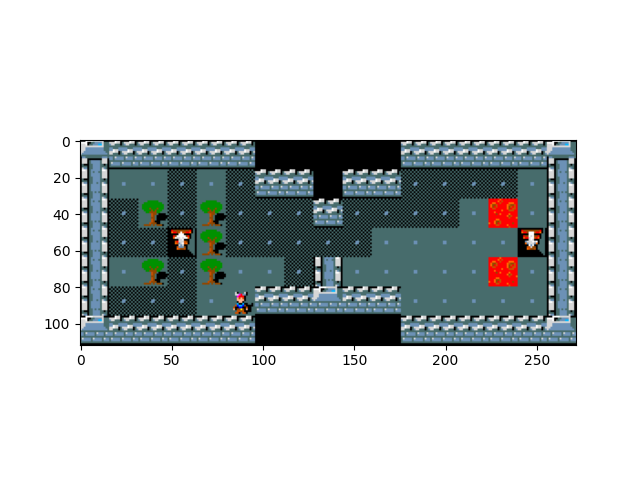
\includegraphics[width=0.18\textwidth]{figures/room-with-lava_FixedAgent/9.png}
	\end{tabular}
	\caption[A fixed agent's trajectory in two Minihack environments]{A fixed agent's trajectory in two Minihack envs (undiscounted, i.e. $\gamma = 1$)}
	\label{fig:room-with-lava_FixedAgent}
\end{figure}



\section{Learning Algorithms}

Dynamic Programming requires a complete \textcolor{blue}{model} of the environment and applies the
Bellman equations to iteratively improve value estimates through \textcolor{green}{bootstrapping}:

\begin{equation}
	\hspace{-20pt}
	\text{Policy Evaluation: } V_{k+1}(s)
	= \sum_a \pi(a|s) Q_k(s, a)
	= \sum_a \pi(a|s) \sum_{s',r} \textcolor{blue}{p(s',r|s,a)} [r + \gamma \textcolor{green}{V_k(s')}]
\end{equation}

\begin{equation}
	\text{Policy Improvement: } \pi'(s)
	= \arg\max_a q_\pi(s, a)
	= \arg\max_a \sum_{s',r} \textcolor{blue}{p(s',r|s,a)} [r + \gamma \textcolor{green}{V_\pi(s')}]
\end{equation}

\begin{equation}
	\text{Value Iteration: } V_{k+1}(s)
	= \max_a \sum_{s',r} Q_k(s, a)
	= \max_a \sum_{s',r} \textcolor{blue}{p(s',r|s,a)} [r + \gamma \textcolor{green}{V_k(s')}]
\end{equation}

\subsection{Model-Free Learning}

While dynamic programming provides optimal solutions when a complete environment model is available, model-free learning is advantageous in scenarios where transition probabilities are unknown, with stochastic dynamics, and when the agent must learn through interaction rather than having access to perfect planning information.

\subsubsection{Monte Carlo (MC) vs. Temporal-Difference (TD) Methods}

Monte Carlo (MC) and Time-Difference (TD) methods are both model-free algorithms.
The key difference lies in how they estimate returns.

MC estimates returns by \textcolor{red}{sampling} complete episodes;
$\delta_t$ is the \textit{return error}.

\begin{equation}
	Q(S_t,A_t) \leftarrow Q(S_t,A_t) + \alpha [ R_{t+1} + \gamma G_{t+1} - Q(S_t,A_t) ], \text{ where } R_{t+1} + \gamma G_{t+1} = \textcolor{red}{G_t}
\end{equation}

TD estimates returns by \textcolor{green}{bootstrapping},
i.e. value estimates $G_{t+1} \textcolor{green}{\approx V(S_{t+1})}$;
in TD(O), $n$-step TD, SARSA and Q-Learning,
$\delta_t$ is the \textit{time-difference error}.

\begin{equation}
	V(S_t) \leftarrow V(S_t) + \alpha [ R_{t+1} + \gamma V(S_{t+1}) - V(S_t) ]
\end{equation}

\begin{equation}
	V(S_t) \leftarrow V(S_t) + \alpha \left[ R_{t+1} + \dots + \gamma^n V(S_{t+n}) - V(S_t) \right]
\end{equation}

\begin{equation}
	Q(S_t,A_t) \leftarrow Q(S_t,A_t) + \alpha [ R_{t+1} + \gamma Q(S_{t+1},A_{t+1}) - Q(S_t,A_t) ]
\end{equation}

\begin{equation}
	Q(S_t,A_t) \leftarrow Q(S_t,A_t) + \alpha [ R_{t+1} + \gamma \max_{a} Q(S_{t+1},a) - Q(S_t,A_t) ]
\end{equation}

\paragraph{Updates}

TD is naturally online, updating at each step as data comes in; and thus fully incremental.
Updates after each step (or $n$ steps for $n$-step TD) can be sufficient for learning,
and more efficient for long episodes.

MC can be implemented incrementally using an incremental average.
This avoids recomputing the complete return $G_t$ for each state-action pair.
Still, by definition, MC must always wait until the end of the episode to update the Q-values.
For longer episodes, MC learning is slower. Compare time in tqdm!

\paragraph{Bias-Variance Trade-off}

MC samples real returns $G_t$, which are unbiased, and with enough experience converge to the true value $v_\pi(s)$.
MC has high variance though as it calculates the return over complete episodes.

The true TD update $v_\pi(S_{t+1})$ is also unbiased, but the TD update is not:
due to bootstrapping, the current estimate $V(S_{t+1})$ may or may not be a correct estimate.
Since there is only one (or finite $n$) step in each TD update, variance is low.
As such, TD methods are more sample-efficient.

\paragraph{Convergence Properties}

Both are guaranteed to converge to the true value function in the limit, i.e. over an infinite number of episodes.

The MC estimate $Q(s, a)$ converges to the true value $q_\pi(s, a)$ with probability $1$,
assuming the returns $G_t$ are bounded and step-sizes $\alpha_t$ satisfy the Robbins-Monro conditions:
$\sum_{t} \alpha_t = \infty, \quad \sum_{t} \alpha_t^2 < \infty$.

TD(0) is biased due to bootstrapping. This bias decreases in the limit.
It converges\footnote{In tabular form. Not always with function approx. Moreover, TD is more sensitive to initial values.} to $v_\pi$ with probability $1$, assuming
the Markov chain induced by $\pi$ is ergodic (i.e. all states are visited infinitely often),
the learning rate $\alpha_t$ satisfies the Robbins-Monro conditions,
and rewards are bounded.

If the number of episodes is finite,
MC converges to the solution with minimum mean squared error (MSE)
between predicted values and observed returns across episodes,
$\sum_{e_i}{\sum_t{(G_t^k - V(s_t^k))^2}}$,
while TD estimates converge to the value function of the Markov model that best explains the observations, i.e. the maximum likelihood.

\paragraph{Markov Property}

This is because TD methods assume that the environment is Markovian - computing
the values of a hypothetical Markov model that maximises the likelihood of the observed transition dynamics.
Therefore, TD methods are more efficient in Markovian environments.
MC methods do not make this assumption, but can be more robust in environments where the Markov property does not apply.

\begin{figure}[!h]
	\centering
	\begin{tabular}{cc}
		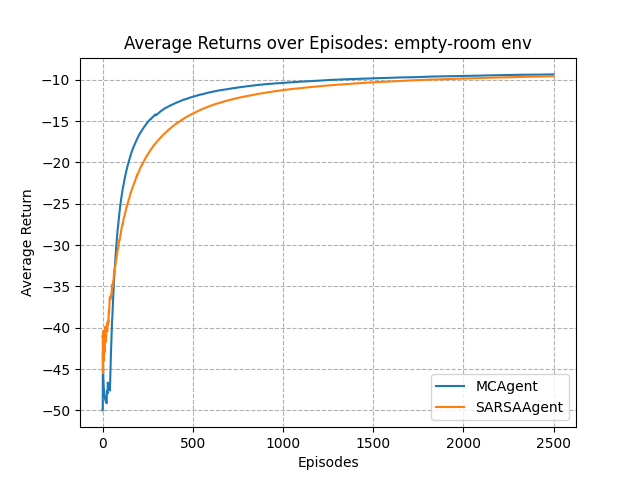
\includegraphics[width=0.48\textwidth]{figures/mc-td-empty-room-5x5.png} &
		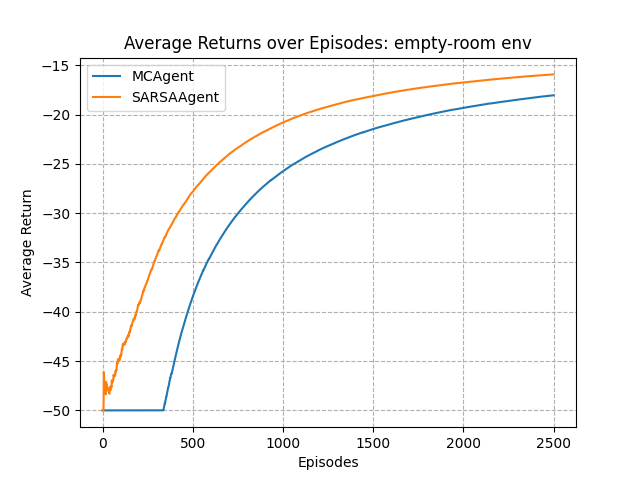
\includegraphics[width=0.48\textwidth]{figures/mc-td-empty-room-7x7.png}                         \\
		(a) $5 \times 5$ grid                                                    & (b) $7 \times 7$ grid
	\end{tabular}
	\caption{Average returns for MC, TD over 2500 episodes in the empty room environment}
	\label{fig:mc-td-empty-room-comparison}
\end{figure}

\begin{figure}[!h]
	\centering
	\begin{tabular}{cc}
		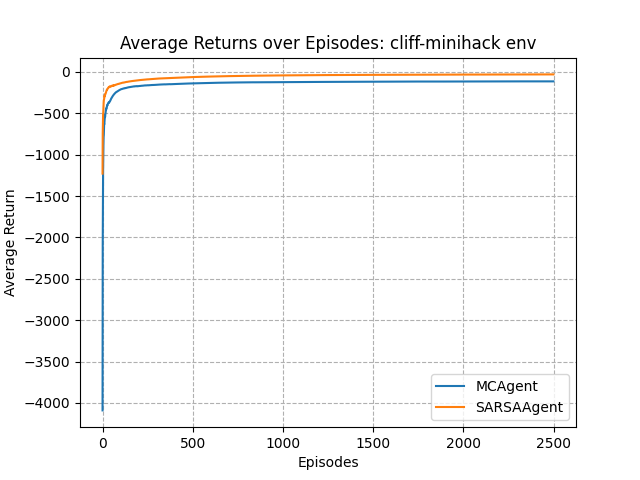
\includegraphics[width=0.48\textwidth]{figures/mc-td-cliff-env.png}
	\end{tabular}
	\caption{Average returns for MC, TD over 2500 episodes in the cliff environment}
	\label{fig:mc-td-cliff-env}
\end{figure}

In summary, bootstrapping in TD methods offers sample efficiency and online learning capability by updating estimates immediately rather than waiting for episode completion,
resulting in lower variance but introducing bias from potentially incorrect value estimates.
This approach may be particularly advantageous in structured environments (like \texttt{EMPTY\_ROOM}) where the Markov property holds strongly,
but also in long episodes (like \texttt{ROOM\_WITH\_MULTIPLE\_MONSTERS}),
and may be less effective in other, shorter, or more outcome-dependent episodes (like \texttt{ROOM\_WITH\_LAVA} or \texttt{CLIFF})
where Monte Carlo's unbiased sampling of complete returns might give better results.

In the simple empty room environment ($5 \times 5$ and $7 \times 7$ grids), both MC and TD methods show comparably good convergence patterns,
but TD demonstrates slightly faster initial learning due to its online updating capability.
The cliff environment reveals a difference:
The TD method achieves consistently higher average returns compared to MC.
This might be because the structured nature of the cliff environment allows TD's bootstrapping to effectively exploit the Markovian structure,
while MC's complete episode sampling may be hindered by high variance in returns caused by the cliff's penalty structure.
The performance gap stays as learning progresses over the course of many episodes,
which means that TD's bias-variance trade-off could be particularly beneficial given the immediate consequences for suboptimal actions.
Additionally, MC's higher variance makes it more sensitive to hyperparameter choices, particularly the learning rate $\alpha$:
since MC updates use the full return $G_t$ which can vary significantly between episodes,
poorly chosen learning rates can lead to unstable learning or slow convergence,
whereas TD's lower-variance single-step updates are generally more robust to suboptimal hyperparameter settings and require less environment-specific tuning in order to perform well.


\subsubsection{First-Visit vs. Every-Visit Monte Carlo Learning}

First-visit MC takes into account only the return observed after the first occurrence of a given state within one episode.
Every-visit MC takes into account all occurrences of a given state in an episode.

\begin{figure}[!h]
	\centering
	\begin{tabular}{cc}
		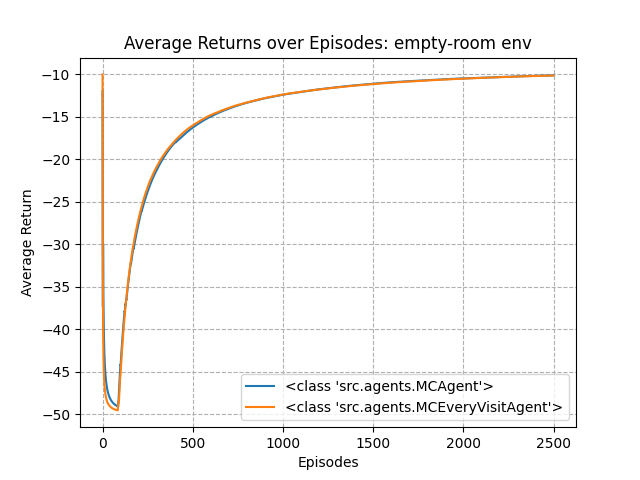
\includegraphics[width=0.48\textwidth]{figures/mc-every-visit-empty-room-5x5.png} &
		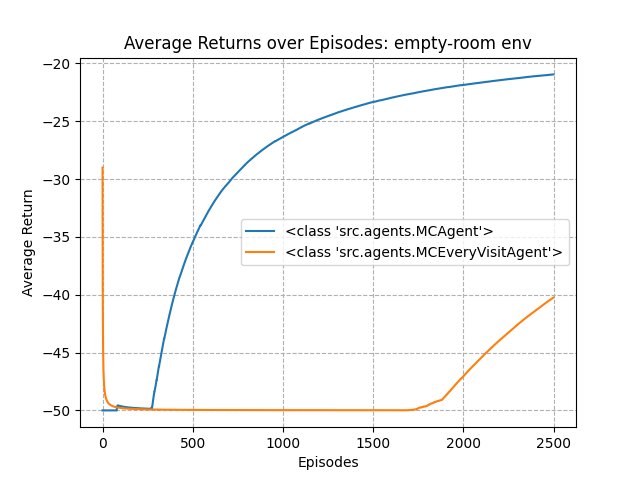
\includegraphics[width=0.48\textwidth]{figures/mc-every-visit-empty-room-7x7.png}                         \\
		(a) $5 \times 5$ grid                                                             & (b) $7 \times 7$ grid
	\end{tabular}
	\caption{Average returns for first, every visit MC over 2500 episodes in the empty room environment}
	\label{fig:mc-every-visit-empty-room}
\end{figure}

First-visit MC is unbiased and converges to the true value function, which makes it theoretically cleaner but potentially slower in environments with frequent state revisits.
It is particularly beneficial in shorter episodes where states may be visited frequently e.g. due to loops or repetitive patterns, as it avoids the correlation issues that arise from multiple updates to the same state within a single episode.

Every-visit MC can extract more data from each episode by utilising all state visits, which can be especially advantageous in longer episodes where states are visited less frequently.
However, every-visit MC introduces correlation between updates within the same episode, as multiple visits to the same state will use the same trajectory tail for computing returns, potentially leading to higher variance in the value estimates.
This correlation can become problematic in environments with frequent state revisits, potentially outweighing the benefits of additional data.

The experimental results illustrate this trade-off: in the $5 \times 5$ environment, both first-visit and every-visit MC perform similarly with only minor differences, suggesting that the correlation effects are manageable.
However, in the larger $7 \times 7$ environment, every-visit MC appears to struggle. This could likely be due to the increased frequency of state revisits in longer episodes amplifying the correlation issues, which makes training less stable and unsuccessful in this case.


\subsubsection{On-Policy vs. Off-Policy Time-Difference Learning}

On-policy methods, such as SARSA, learn the value of the policy currently being followed, e.g. $\epsilon$-greedy.
The update targets actions that are already taken, thus including exploratory actions.
The policy is improved gradually and converges to the optimal ($\epsilon$-greedy) policy.

\begin{equation}
	A_{t+1} \sim \pi_{\epsilon\text{-greedy}}(a \mid S_{t+1})
\end{equation}

Off-policy methods, such as Q-learning, learn the value of an optimal target policy
while following a different behaviour policy (usually $\epsilon$-greedy for exploration), which enables reuse of past experience and is more sample-effiient.
The update of that target policy uses the greedy action, $\pi_\text{greedy}(a \mid s)$!

\begin{equation}
	\hspace{-5pt}
	Q(S_t,A_t) \leftarrow Q(S_t,A_t) + \alpha [ R_{t+1} + \gamma Q(S_{t+1}, \hat{a}) - Q(S_t,A_t) ]
	, \quad
	\hat{a} = \arg\max_{a} Q(S_{t+1}, a)
\end{equation}

\begin{figure}[!h]
	\centering
	\begin{tabular}{cc}
		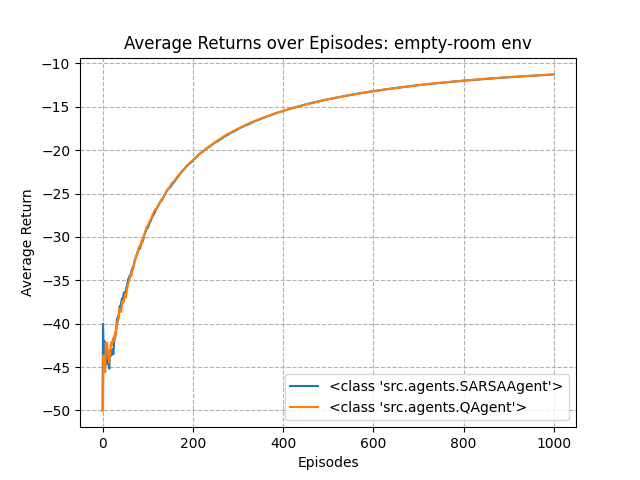
\includegraphics[width=0.48\textwidth]{figures/on-off-policy-empty-room.png} &
		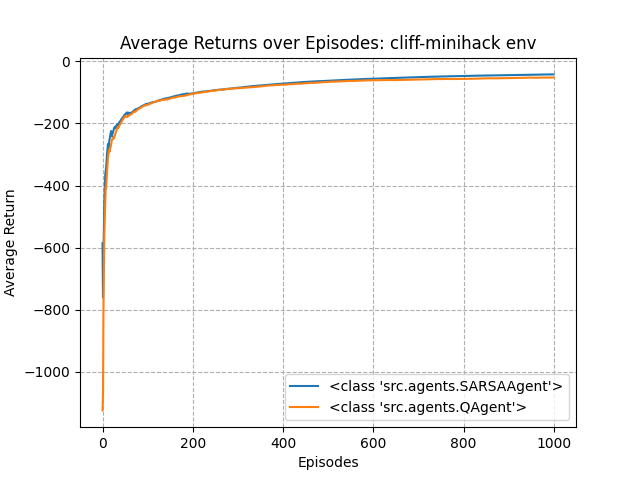
\includegraphics[width=0.48\textwidth]{figures/on-off-policy-cliff.png}                      \\
		(a) Empty room env                                                           & (b) Cliff env
	\end{tabular}
	\caption{Average returns for on, off-policy TD over 1000 episodes in the empty room, cliff environments}
	\label{fig:on-off-policy}
\end{figure}

In the CLIFF environment, SARSA and Q-Learning agents converge to different strategies.
This is due to the fact that SARSA uses on-policy control while Q-Learning uses off-policy control:
SARSA on-policy learns the less risky strategy of avoiding the cliff;
Q-Learning off-policy is able to explore in parallel to learning the optimal policy,
and therefore manages to learn the riskier but optimal (in terms of reward) strategy.
This is also reflected in the returns where Q-Learning would appear to be doing worse:
this is because in off-policy learning, the agent learns about the greedy policy while following an exploratory policy but it is not taken into account that the agent is actually exploring; executing the greedy strategy however it becomes visible that Q-Learning has found the shorter, more optimal path.

\paragraph{Expected SARSA and Double Q-Learning}

There are also extensions and improvements of the SARSA\footnote{
	Expected SARSA is a hybrid approach that computes the expected value over the next state's action values, weighted by the current policy.
	This weighted average reduces variance: $Q(S_t,A_t) \leftarrow Q(S_t,A_t) + \alpha [ R_{t+1} + \gamma \sum_a{\pi(a \mid s) Q(S_{t+1}, a)} - Q(S_t,A_t) ]$.
} and Q-Learning
% \footnote{
% 	In Q-learning (and Deep Q-Learning) there is \textit{maximisation bias} because
% 	the same samples are used both to select, $A^* = \arg\max_a Q(S_{t+1}, a)$, and evaluate the best action.
% 	In contrast, with SARSA, the action selected from the current policy is used for evaluation.
% 	There is no max operation, and therefore no maximisation bias.
% 	(Although of course all TD methods, incl. SARSA, exhibit bias due to bootstrapping.)

% 	The maximum of multiple random estimates can overestimate the true maximum.
% 	Double Q-learning maintains two value functions, $Q_1$ and $Q_2$,
% 	thus decoupling action selection from value estimation.
% 	Each Q-function is updated with 50\% probability using the action selected by the other.
% 	This mitigates bias in the estimate $\mathbb{E}[Q_2(A^*)] = q(A^*)$ and can improve stability in learning.
% 	\nopagebreak
% 	\begin{equation}
% 		A^* = \arg\max_a Q_1(S_{t+1}, a), \quad
% 		Q_1(S_t, A_t) \leftarrow Q_1(S_t, A_t) + \alpha \left[ R_{t+1} + \gamma Q_2(S_{t+1}, A^*) - Q_1(S_t, A_t) \right]
% 	\end{equation}

% 	Q-learning is not well-suited for problems with very large numbers of states and actions because it requires maintaining a Q-table of size $|S| \times |A|$, which becomes computationally and memory-wise intractable as these dimensions grow.
% 	Function approximation (e.g., neural networks) is needed for such scenarios, leading to Deep Q-Learning.
% }
algorithms.
They are not experimented with here but could be interesting to try in some of the more complex environments.
In particular, expected SARSA is found to find an intermediate policy - not as conservative and not as optimal but right in the middle - between SARSA and Q-Learning in the cliff environment!

\paragraph{Off-Policy and On-Policy Monte Carlo Methods}

MC is only implemented on-policy. There also exists off-policy MC, although it is not implemented.
Only two on-policy (SARSA) and off-policy (Q-Learning) TD methods are considered.

\subsubsection{Exploration vs. Exploitation}

To discover optimal policies, exploration of all the state-action pairs is necessary.
To get high returns, exploitation of known high-value pairs is needed.
This is known as the exploration-exploitation trade-off.

$\epsilon$-greedy action selection\footnote{
	$\epsilon$-greedy is the most greedy policy of the $\epsilon$-soft class of policies, for which
	all actions are selected at least $\pi(a \mid s) \geq \frac{\epsilon}{\lvert A(s) \rvert}$.
	Setting $\epsilon = 0$ makes the policy fully greedy.
} is a common technique for handling the exploration-exploitation trade-off.
Exploring a random action occurs with probability $\epsilon$;
the greedy action is exploited with probability $1 - \epsilon$.

On-policy methods are affected more strongly in their learning behaviour by exploration,
because they learn the value of the policy being followed.

Off-policy methods decouple behaviour and learning by separating these two concerns in
a behaviour (e.g. $\epsilon$-greedy) and a target (typically greedy) policy.
Off-policy methods are therefore less sensitive to the choice of \(\epsilon\),
as the update of the target policy is not affected
by the amount of exploration performed by the behaviour policy.

\begin{figure}[!h]
	\centering
	\begin{tabular}{ccc}
		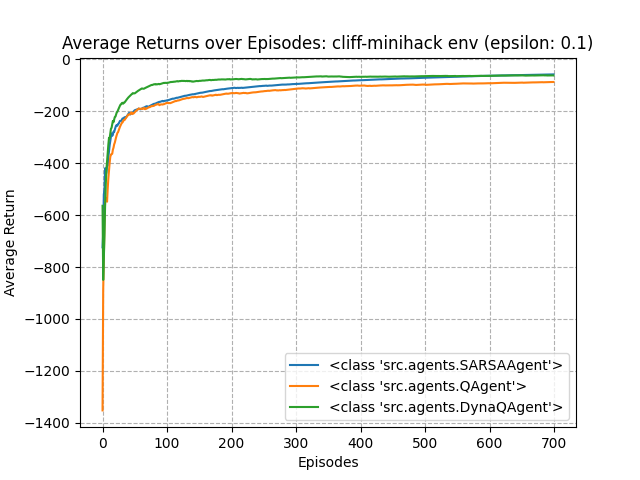
\includegraphics[width=0.32\textwidth]{figures/epsilon-0-1-cliff.png} &
		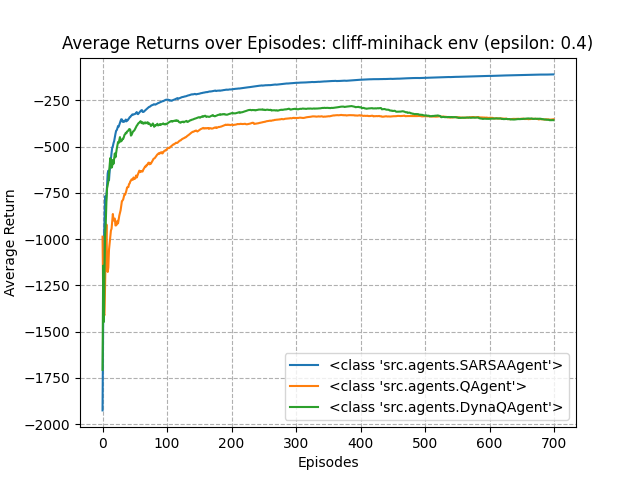
\includegraphics[width=0.32\textwidth]{figures/epsilon-0-4-cliff.png} &
		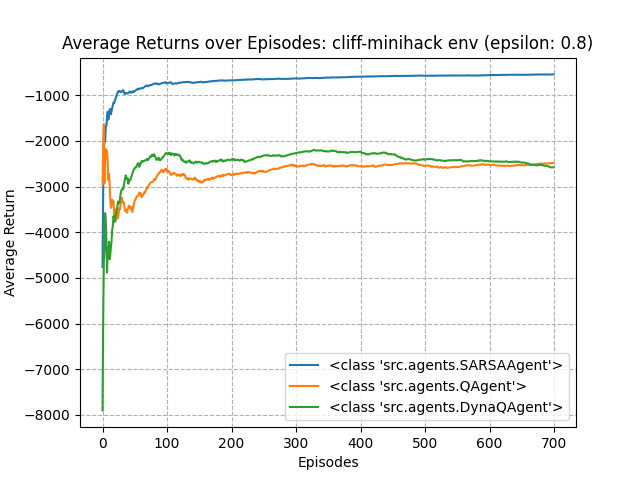
\includegraphics[width=0.32\textwidth]{figures/epsilon-0-8-cliff.png}                                               \\
		(a) $\epsilon = 0.1$                                                  & (b) $\epsilon = 0.4$ & (c) $\epsilon = 0.8$
	\end{tabular}
	\caption{Average returns for $\epsilon = 0.1, 0.4, 0.8$ over 700 episodes in the cliff environment}
	\label{fig:epsilon-cliff}
\end{figure}

With a high learning rate, Q-Learning and Dyna-Q still manage to learn the optimal policy.
SARSA, even more conservatively, learns to stay away even farther from the cliff.


\subsubsection{The Learning Rate}

The \textbf{learning rate} $\alpha \in (0,1]$ is the step size of the updates,
$Q(s, a) \leftarrow Q(s, a) + \alpha \delta_t$.

Hyperparameter tuning of the learning rate is implemented.
A \textit{high learning rate} (e.g., \(\alpha = 1.0\)) allows rapid incorporation of new information but can lead to high variance and oscillations in the value estimates due to the stochasticity of rewards and transitions.
A \textit{low learning rate} results in smaller incremental updates, producing slower but more stable learning.

\paragraph{Decaying vs. Constant \(\alpha\)}

The Robbins-Monro conditions for convergence,
$\sum_{t=1}^\infty \alpha_t = \infty$ and $\sum_{t=1}^\infty \alpha_t^2 < \infty$,
imply a decrease in step size over time.
The implication is to balance learning with diminishing variance
under convergence assumptions (ergodicity, sufficient exploration, bounded rewards).
If the environment keeps changing, a fixed learning rate enables continued learning,
although the policy may not converge then.


\subsection{\texorpdfstring{$\epsilon$}{e}-Scheduling}

In the CLIFF environment, as previously discussed,
SARSA learns about the policy it's actually following (including exploratory moves).
Q-Learning learns about the optimal policy directly, ignoring exploratory moves.
This makes SARSA more conservative in dangerous environments (it accounts for exploration risks).
Q-Learning can be more aggressive by learning optimal values independent of exploration strategy.

A decreasing scheduling of the $\epsilon$ value during learning
(i.e. decreasing the value of $\epsilon$ after each episode) is implemented using
linear decay,
where $\epsilon_\text{start}$ is the initial (maximal) $\epsilon$ value,
$\epsilon_\text{end}$ is the minimal $\epsilon$ value (e.g. $0$),
$k$ is the episode index, and
$\max\{k\}$ is the maximum number of episodes used in the decay.

\begin{equation}
	\epsilon_k = \epsilon_\text{start} - k \frac{\epsilon_\text{start} - \epsilon_\text{end}}{\max\{k\}}
\end{equation}

% TODO: Plot a sample trajectory using the target policy at different stages of the learning
% (i.e. at different episodes $k$) and explain the observed behaviour.

In SARSA the target policy (i.e. what the agent aims to learn)
is still the $\epsilon$-greedy policy (on-policy), while
in Q-learning the target policy is always the greedy policy (off-policy).
This means SARSA learns the value of the epsilon-greedy policy, including exploratory actions.
In Q-Learning, the target policy always selects the best action, while the behavior policy occasionally explores.
Q-learning therefore learns the value of the optimal policy, regardless of the actual behavior during learning.

When epsilon decays to a small value, SARSA's learned policy still accounts for that small amount of exploration.
\textit{Q-learning converges to the optimal deterministic policy regardless of epsilon's final value}.

Moreover, $\epsilon$-scheduling can speed up convergence.
A high initial $\varepsilon$ allows better exploration early on which helps avoid suboptimal policies.
However, it is important to note that low decay can mean longer convergence time, since you keep exploring, incl. bad actions;
fast decay reduces unnecessary exploration, but may lead to premature convergence to suboptimal policies.

Essentially, decreasing $\varepsilon$ means having exploited enough and trusting the policy to act greedily from here on.
Whereas decreasing $\alpha$ meant trusting the value updates more and updating them less drastically.


\subsection{Model-Based Learning}

Planning uses a model of the environment to compute value estimates and select actions,
while learning improves value estimates directly through interaction.
The two techniques can be unified by planning in an inner loop using simulated experience,
and learning in an outer loop using real interaction.

% Distributional models (like those in DP) represent full transition and reward probabilities, allowing flexible sampling but requiring strong assumptions regarding or knowledge of the environment.
% Sample models (like in MC methods) rely on observed experience and are easier to build but less complete.

Dyna integrates model learning, planning, and direct reinforcement learning
by constructing a model from observed $(s, a, r, s')$ tuples (assuming determinism!).
Then, after each real interaction, $n$ simulated updates using the internal model are performed.
Planning occurs in the background, decoupled from action selection.\footnote{
	Decision-time planning (higher latency!), e.g. heuristic search, is an action selection method for the current local state only.
	Greedy action selection is the base form of heuristic search.
	Rollout algorithms use a MC approach for decision-time planning: sampling entire trajectories and backing up values (MCTS: selection, expansion, simulation, backup).
}

Dyna thus
(a) improves the model through learning,
(b) indirectly improves the policy through planning, and
(c) directly improves the policy by using simulated experience to perform updates,
accelerating policy improvement with fewer real interactions.

\begin{figure}[!h]
	\centering
	\begin{tabular}{cc}
		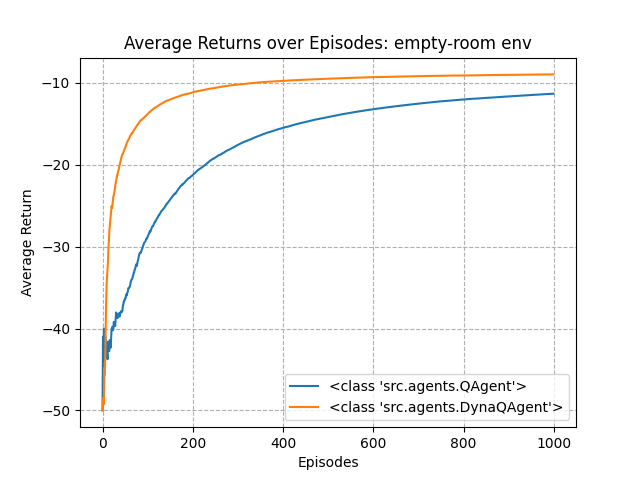
\includegraphics[width=0.48\textwidth]{figures/dyna-q-empty-room.png} &
		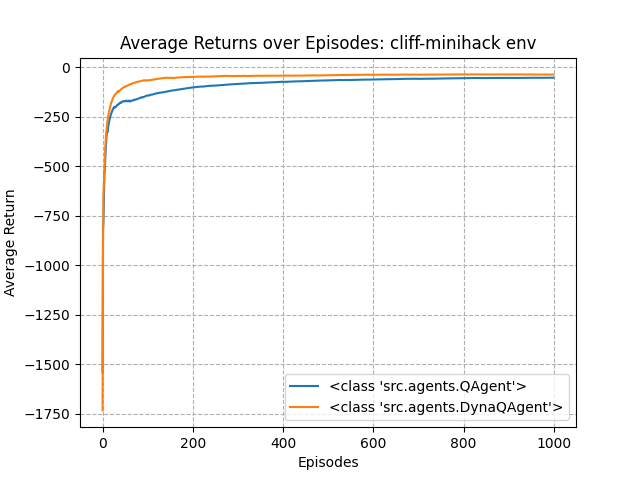
\includegraphics[width=0.48\textwidth]{figures/dyna-q-cliff.png}                      \\
		(a) Empty room env                                                    & (b) Cliff env
	\end{tabular}
	\caption{Average returns for Dyna-Q, Q-Learning over 1000 episodes in the empty room, cliff environments}
	\label{fig:dyna-q}
\end{figure}

\paragraph{Dyna-Q+}

Dyna-Q+ extends Dyna-Q with an exploration bonus:
each state-action pair is rewarded based on how long ago it was last visited, $R + \kappa \sqrt{\tau}$.
This encourages exploration of forgotten or under-sampled transitions.
\textit{Dyna-Q+ performs better than Dyna-Q in environments where the dynamics change over time or where new, rewarding regions can appear}.
Dyna-Q+ is not implemented here,
but may yield improvements over Dyna, for example, in the room with monsters, which is subject to continuous change.


\section{Deep Learning Algorithms}

Reinforcement learning with function approximation allows scaling to large or continuous state and action spaces,
where tabular methods become infeasible.
Deep RL uses deep neural networks (DNNs) as function approximators for value functions, policies, or both.
These networks are trained by minimising a loss function, $\min_w{\frac{1}{\lvert D \rvert} \sum_{(x, y) \in D}{\ell(y, f(x; w))}}$.

% However, unlike supervised learning, the data in RL are not i.i.d.:
% consecutive states and actions are often correlated (which can cause overfitting or forgetting about previous states), and bootstrapping causes moving targets $y = r + \gamma \max_a{Q(s', a; \theta)}$.
% These characteristics lead to instability and inefficiency, known as the deadly triad:
% bootstrapping, off-policy learning, and function approximation.

% A solution to data correlation is experience replay: storing experience in a buffer, and updating the network on a sampled minibatch from the entire buffer.
% A solution to moving targets is to use a target network, e.g. a two Q-network with a fast parameter $\theta$ and a slow parameter $\theta^-$
% with a soft update on every training step,
% $\theta^-_{t+1} = \tau \theta_t + (1-\tau)\theta_t^-, \, \tau \in [0, 1]$, e.g. $\tau = 0.001$,
% and a hard update every $M$ training steps, $\theta^- = \theta_t$.

% Experience replay breaks correlation by storing transitions and sampling uniformly.
% Target networks stabilise bootstrapping by slowing changes in the target:
% using soft updates
% $\theta^-_{t+1} = \tau \theta_t + (1-\tau)\theta_t^-$
% or hard updates $\theta^- = \theta_t$ every $M$ steps.
% Batch updates maximally utilise experiences.
% With experience replay, updates are performed not on online experience but on minibatches of the stored experience.

\subsection{Deep Q-Learning}

DQN is a \textit{value-based} DRL method that combines Q-learning with neural networks
to approximate the optimal action-value function, $Q^*(s, a)$.
The Q-network is updated by minimising the Bellman error using experience replay and a target network.
During experience replay, an exploratory policy (e.g. $\epsilon$-greedy) is used, and transitions $(s_t, a_t, r_t, s_{t+1})$ are stored.
To reduce overestimation bias in Q-learning due to the max operator, Double Q-Learning uses the current network to select the action and the target network to evaluate it.
The target network can be used as a second value function but, like in Double Q-Learning,
selection needs to be decoupled from evaluation to avoid maximisation bias.

% \begin{table}[h!]
%     \centering
%     \begin{tabular}{|c|c|}
%         \hline
%         Q-Learning with Value Approximation
% 		& $y_{\textcolor{green}{\theta}} = R_{t+1} + \gamma \max_a{\hat{q}(S_{t+1}, a; \textcolor{green}{\theta})}$ \\
% 		\hline
% 		Deep Q-Learning
% 		& $y_{\textcolor{green}{\theta}} = R_{t+1} + \gamma \max_a{\hat{q}(S_{t+1}, a; \textcolor{blue}{\theta^-})}$ \\
% 		\hline
% 		Double Deep Q-Learning
% 		& $y_{\textcolor{green}{\theta}} = R_{t+1} + \gamma \hat{q}(S_{t+1}, \max_a{\hat{q}(S_{t+1}, a; \textcolor{green}{\theta})}; \textcolor{blue}{\theta^-})$ \\
% 		\hline
%     \end{tabular}
%     \caption{Q-Learning variants with target networks and their update targets}
%     \label{tab:dqn}
% \end{table}

% The Q-value function $\hat{q}(S_t, A_t; \bm{w})$ is a neural network
% that takes as input a vector representation of state $S_t$
% and outputs a categorical distribution, e.g. softmax, with $n = \lvert A_t \rvert$ parameters.
% To improve generalisation and efficiency, the Q-function can be factorised as follows, and which
% separates state-value and action-advantage learning:
% in some states, the action may not matter that much, e.g. a red light;
% learning state value and action advantage can enable
% faster learning in value-dominant states
% and better generalisation across actions.

% \begin{equation}
% 	Q(s, a) = V(s) + \bigg( A(s, a) - \frac{1}{A} \sum_{a'}{A(s, a')} \bigg)
% \end{equation}

\subsection{Actor-Critic Methods}

Policy gradient methods are policy-based methods optimise the parameters of a stochastic policy $\pi(a \mid s; \bm{\theta})$ directly via gradient ascent:

\begin{equation}
	\bm{\theta}_{t+1} \leftarrow \bm{\theta}_t + \alpha G_t \nabla \log{\pi(A_t \mid S_t; \bm{\theta})}
\end{equation}

% This is the REINFORCE algorithm, which uses the sampled return $G_t$ to estimate the policy gradient. It enables continuous actions and avoids the need for value functions, but suffers from high variance.
% A baseline $b(S_t)$ can reduce variance without biasing the gradient:

% \begin{equation}
% 	\bm{\theta}_{t+1} \leftarrow \bm{\theta}_t + \alpha [G_t - b(S_t)] \nabla \log{\pi(A_t \mid S_t; \bm{\theta})}
% \end{equation}

% Bootstrapping the return is called a \textit{critic}, often a value function $v(S; \bm{w})$:

% \begin{equation}
% 	\bm{\theta}{t+1} \leftarrow \bm{\theta}t + \alpha [R_{t+1} + \gamma v(S_{t+1}) - v(S_t)] \nabla \log{\pi(A_t \mid S_t)}
% \end{equation}

The combination of an actor (policy) and critic (value function) forms Actor-Critic methods, e.g. A2C, A3C, PPO, DDPG. These methods reduce variance in policy gradients and support more stable learning.

% Policy gradient methods learn the policy directly.
% Therefore, exploration is determined by the stochasticity of the parametric family, rather than externally determined.
% The stochasticity of a policy is its KL distance from a random policy which is proportional to its negative entropy,
% $D_\text{KL}[\pi(a \mid s) \Vert \pi_\text{random}(a \mid s)] \propto -H(\pi)$.
% Stochasticity can be encouraged by maximal entropy regularisation.

% Policy entropy also matters for exploration. Encouraging stochasticity can be formalised via entropy regularisation:

% \begin{equation}
% 	D_\text{KL}[\pi(a \mid s) \Vert \pi_\text{random}(a \mid s)] \propto -H(\pi)
% \end{equation}

\subsection{Comparison}

Both DQN and PPO are implemented using Stable Baselines3.
The environments provide observations as character-based grids, which are \textit{encoded numerically} using a mapping: agent=1, free space=0, goal=2, start=3.
The encoding implemented is crucial for transforming the symbolic grid representation into numerical arrays suitable for neural network processing - in order for the network to be able to learn.
Both are more difficult to train. \\

PPO demonstrates faster initial learning due to its policy gradient approach and ability to take multiple gradient steps per data collection phase.
DQN is a value-based method and requires more exploration episodes. But once converged DQN can achieve very stable final performance.
PPO's advantage lies in its sample efficiency during early training phases, while DQN is off-policy which allows it to learn from a broader set of samples in its replay buffer. \\

Tabular Q-learning provides \textit{exact} value function representation and \textit{guarantees convergence}.
For small environments like the ones experimented with here it is therefore sufficient to achieve good performance and preferable because it is a much more lightweight algorithm.
However, it suffers from the curse of dimensionality, i.e. it becomes computationally intractable for large state spaces.
Deep Q-learning overcomes scalability limitations through function approximation, and despite approximation errors and potential instability from the deadly triad (bootstrapping, off-policy learning, function approximation)is more practical for complex, real-world problems.


\newpage
\nocite{*}
\printbibliography

\end{document}
